\documentclass[]{book}
\usepackage{lmodern}
\usepackage{amssymb,amsmath}
\usepackage{ifxetex,ifluatex}
\usepackage{fixltx2e} % provides \textsubscript
\ifnum 0\ifxetex 1\fi\ifluatex 1\fi=0 % if pdftex
  \usepackage[T1]{fontenc}
  \usepackage[utf8]{inputenc}
\else % if luatex or xelatex
  \ifxetex
    \usepackage{mathspec}
  \else
    \usepackage{fontspec}
  \fi
  \defaultfontfeatures{Ligatures=TeX,Scale=MatchLowercase}
\fi
% use upquote if available, for straight quotes in verbatim environments
\IfFileExists{upquote.sty}{\usepackage{upquote}}{}
% use microtype if available
\IfFileExists{microtype.sty}{%
\usepackage[]{microtype}
\UseMicrotypeSet[protrusion]{basicmath} % disable protrusion for tt fonts
}{}
\PassOptionsToPackage{hyphens}{url} % url is loaded by hyperref
\usepackage[unicode=true]{hyperref}
\hypersetup{
            pdftitle={Conceptual and methodological problems with bias detection and avoidance in natural language processing},
            pdfauthor={Alicja Dobrzeniecka},
            pdfborder={0 0 0},
            breaklinks=true}
\urlstyle{same}  % don't use monospace font for urls
\usepackage{color}
\usepackage{fancyvrb}
\newcommand{\VerbBar}{|}
\newcommand{\VERB}{\Verb[commandchars=\\\{\}]}
\DefineVerbatimEnvironment{Highlighting}{Verbatim}{commandchars=\\\{\}}
% Add ',fontsize=\small' for more characters per line
\usepackage{framed}
\definecolor{shadecolor}{RGB}{248,248,248}
\newenvironment{Shaded}{\begin{snugshade}}{\end{snugshade}}
\newcommand{\KeywordTok}[1]{\textcolor[rgb]{0.13,0.29,0.53}{\textbf{#1}}}
\newcommand{\DataTypeTok}[1]{\textcolor[rgb]{0.13,0.29,0.53}{#1}}
\newcommand{\DecValTok}[1]{\textcolor[rgb]{0.00,0.00,0.81}{#1}}
\newcommand{\BaseNTok}[1]{\textcolor[rgb]{0.00,0.00,0.81}{#1}}
\newcommand{\FloatTok}[1]{\textcolor[rgb]{0.00,0.00,0.81}{#1}}
\newcommand{\ConstantTok}[1]{\textcolor[rgb]{0.00,0.00,0.00}{#1}}
\newcommand{\CharTok}[1]{\textcolor[rgb]{0.31,0.60,0.02}{#1}}
\newcommand{\SpecialCharTok}[1]{\textcolor[rgb]{0.00,0.00,0.00}{#1}}
\newcommand{\StringTok}[1]{\textcolor[rgb]{0.31,0.60,0.02}{#1}}
\newcommand{\VerbatimStringTok}[1]{\textcolor[rgb]{0.31,0.60,0.02}{#1}}
\newcommand{\SpecialStringTok}[1]{\textcolor[rgb]{0.31,0.60,0.02}{#1}}
\newcommand{\ImportTok}[1]{#1}
\newcommand{\CommentTok}[1]{\textcolor[rgb]{0.56,0.35,0.01}{\textit{#1}}}
\newcommand{\DocumentationTok}[1]{\textcolor[rgb]{0.56,0.35,0.01}{\textbf{\textit{#1}}}}
\newcommand{\AnnotationTok}[1]{\textcolor[rgb]{0.56,0.35,0.01}{\textbf{\textit{#1}}}}
\newcommand{\CommentVarTok}[1]{\textcolor[rgb]{0.56,0.35,0.01}{\textbf{\textit{#1}}}}
\newcommand{\OtherTok}[1]{\textcolor[rgb]{0.56,0.35,0.01}{#1}}
\newcommand{\FunctionTok}[1]{\textcolor[rgb]{0.00,0.00,0.00}{#1}}
\newcommand{\VariableTok}[1]{\textcolor[rgb]{0.00,0.00,0.00}{#1}}
\newcommand{\ControlFlowTok}[1]{\textcolor[rgb]{0.13,0.29,0.53}{\textbf{#1}}}
\newcommand{\OperatorTok}[1]{\textcolor[rgb]{0.81,0.36,0.00}{\textbf{#1}}}
\newcommand{\BuiltInTok}[1]{#1}
\newcommand{\ExtensionTok}[1]{#1}
\newcommand{\PreprocessorTok}[1]{\textcolor[rgb]{0.56,0.35,0.01}{\textit{#1}}}
\newcommand{\AttributeTok}[1]{\textcolor[rgb]{0.77,0.63,0.00}{#1}}
\newcommand{\RegionMarkerTok}[1]{#1}
\newcommand{\InformationTok}[1]{\textcolor[rgb]{0.56,0.35,0.01}{\textbf{\textit{#1}}}}
\newcommand{\WarningTok}[1]{\textcolor[rgb]{0.56,0.35,0.01}{\textbf{\textit{#1}}}}
\newcommand{\AlertTok}[1]{\textcolor[rgb]{0.94,0.16,0.16}{#1}}
\newcommand{\ErrorTok}[1]{\textcolor[rgb]{0.64,0.00,0.00}{\textbf{#1}}}
\newcommand{\NormalTok}[1]{#1}
\usepackage{longtable,booktabs}
% Fix footnotes in tables (requires footnote package)
\IfFileExists{footnote.sty}{\usepackage{footnote}\makesavenoteenv{long table}}{}
\usepackage{graphicx,grffile}
\makeatletter
\def\maxwidth{\ifdim\Gin@nat@width>\linewidth\linewidth\else\Gin@nat@width\fi}
\def\maxheight{\ifdim\Gin@nat@height>\textheight\textheight\else\Gin@nat@height\fi}
\makeatother
% Scale images if necessary, so that they will not overflow the page
% margins by default, and it is still possible to overwrite the defaults
% using explicit options in \includegraphics[width, height, ...]{}
\setkeys{Gin}{width=\maxwidth,height=\maxheight,keepaspectratio}
\IfFileExists{parskip.sty}{%
\usepackage{parskip}
}{% else
\setlength{\parindent}{0pt}
\setlength{\parskip}{6pt plus 2pt minus 1pt}
}
\setlength{\emergencystretch}{3em}  % prevent overfull lines
\providecommand{\tightlist}{%
  \setlength{\itemsep}{0pt}\setlength{\parskip}{0pt}}
\setcounter{secnumdepth}{5}
% Redefines (sub)paragraphs to behave more like sections
\ifx\paragraph\undefined\else
\let\oldparagraph\paragraph
\renewcommand{\paragraph}[1]{\oldparagraph{#1}\mbox{}}
\fi
\ifx\subparagraph\undefined\else
\let\oldsubparagraph\subparagraph
\renewcommand{\subparagraph}[1]{\oldsubparagraph{#1}\mbox{}}
\fi

% set default figure placement to htbp
\makeatletter
\def\fps@figure{htbp}
\makeatother

\usepackage{todonotes}

\title{Conceptual and methodological problems with bias detection and avoidance
in natural language processing}
\author{Alicja Dobrzeniecka}
\date{2021-06-08}

\begin{document}
\maketitle

{
\setcounter{tocdepth}{5}
\tableofcontents
}
\chapter*{Preface}\label{preface}
\addcontentsline{toc}{chapter}{Preface}

Test

\chapter{Introduction}\label{introduction}

\textbf{state the general topic and give some background}

Natural language processing (NLP) is a subfield of computer science that
processes and analyzes language in text and speech with the use of
modern programming methods. It has practical applications in everyday
life as it concerns tasks such as email filters, smart assistants,
search results, language translations, text analytics and so on. Models
used to accomplish these tasks need a lot of data to learn from. This
data originates from humans activities and historical recordings like
texts, messages, speeches. It turns out that in the learning process
these models can learn implicit biases that reflect harmful
stereotypical thinking still present in modern societies. One can find
methods that aim at identifying hidden biases and/or try to remove them
by modifying the models explicitly. There are many different types of
models in NLP depending on a task that they ought to solve. However all
of them need as an input words represented as numerical values and this
is accomplished with word embedding models. The biases seem to have
their primary source in the way the words are assigned the numerical
values. \newline

\textbf{review of the literature related to the topic}

There is a bunch of literature available on the topic of bias detection
and mitigation in NLP models. Bolukbasi2016Man focuses on gender biases
that may be observable while investigating the representation of job
occupations and gender in terms of their assigned numerical values. The
authors apply cosine similarity measurement to investigate the
phenomenon where jobs stereotypically associated with a given gender are
in fact in the model situated closer to this gender.

Caliskan2017Semantics touches upon the topic of biases regarding race
and gender. They apply knowledge from well-known psychological studies
like Implicit Association Test to research the relation between human
stereotypical thinking and model learnt biases to discover close
relationship between these two. For the evaluation they use Word
Embedding Association Test (WEAT) and the Word Embedding Factual
Association Test (WEFAT).

manzini2019black proposes novel way of using a cosine similarity method
to get the information on assumed resemblance between words. They
investigate an approach that enables to measure the bias for a class
(like gender, religion, race) and express the final result with only one
averaged number. \newline

\textbf{define the terms and scope of the topic}

It is worth noticing the general distinction of biases mentioned in
Caliskan2017Semantics. They refer to the publication concerning Implicit
Association Test Greenwald et al., 1998) where certain baseline of bias
phenomenon was introduced. Namely it seems that humans naturally exhibit
some biases and that not always bring social concern. One can imagine
the intuitive associations between for example insects and flowers, and
the feelings of pleasantness or unpleasantness. In general people would
rather associate flowers with feeling pleasant than insects and this
preference could be named a bias or prejudice in some direction. However
this type of preference does not cause an uproar and it is rather
morally neutral case. Unfortunately there are other biases and
prejudices that directly influence the quality of other people's lives
and therefore they should be taken care of.

One can find a bunch of various definitions trying to capture what bias
and fairness actually are. With the choice of the definition,
implications into the real-life applications may change as well as it
was pointed out in Mehrabi2019Survey. They mark out that there exist
different types of biases, the list if long but among others there are
historical bias, representation bias, measurement bias. This indicates
how complex the process itself is. Without the proper understanding and
awareness of the problem, people are prone to unconsciously sustain this
phenomenon.

In the article one can also find the distinction on different types of
discrimination, some of them will be shortly described. It is worth
first mentioning that protected attributes are those qualities, traits
or characteristics that one cannot, according to the law, discriminated
against. Direct discrimination refers to the situation when protected
attributes of individuals explicitly result in non-favorable outcomes
toward them. In contrast in indirect discrimination individuals appear
to be treated equally but anyway they end up being treated unjustly due
to the hidden effects of biases towards their protected attributes.
Systemic discrimination takes place when policies, customs or behaviors
that result from certain culture or organizational structure lead to
discrimination against some groups of people. Finally, very common
statistical discrimination refers to using average group statistics to
judge person belonging to the group.

The topic of discrimination is entangled with another concept which is
fairness. It is essential to grasp some concepts of fairness to take
them into consideration while designing implementation of some machine
learning model. In Mehrabi2019Survey one may notice that depending on
the context and application different definitions may be applied.
\newline

\textbf{outline the current situation} The most popular methods focus on
comparing the similarity between words from protected groups and those
that are considered to be stereotypical or harmful in some way. One can
find in this group methods such as euclidean distance, dot product or
cosine similarity. There are also other ways to detect the effects of
biases. For example through the investigation of the model performance
on certain tasks that validate if the model returns some values
independently on gender or race or not. \newline

\textbf{evaluate the current situation (advantages/ disadvantages) and identify the gap}

In the currently used methods (like cosine similarity) the values of
similarity are often aggregated in a way that may lead to false
conclusions. For example due to the averaging of values and the lack of
confidence interval information. \newline

\textbf{identify the importance of the proposed research} One can find a
number of articles on negative real-life implications resulting from the
presence of unaddressed biases in the machine learning models. \newline

\textbf{state the research problem/ questions}

In the paper we indicate how current methods used to detect biases in
natural language models are limited in terms of confidence interval.
\newline

\textbf{state the research aims and/or research objectives}

Our research tries to answer the question of how to enhance the current
way in which the bias detection is performed to make sure that it is
methodologically valid. \newline

\textbf{state the hypotheses}

Our hypothesis is that there can be greater understanding of data and
bias implications when confidence interval and Bayesian method are
applied to the methodology. \newline
<!-- \textbf{outline the order of information in the thesis} -->

\textbf{outline the methodology}

To discuss!

\chapter{Bayesian analysis of cosine-based
bias}\label{bayesian-analysis-of-cosine-based-bias}

We start with loading the libraries needed for the analysis.

\footnotesize

\begin{Shaded}
\begin{Highlighting}[]
\KeywordTok{library}\NormalTok{(ggplot2)}
\KeywordTok{library}\NormalTok{(ggthemes)}
\KeywordTok{library}\NormalTok{(rethinking)}
\KeywordTok{library}\NormalTok{(tidyverse)}
\KeywordTok{library}\NormalTok{(ggpubr)}
\KeywordTok{library}\NormalTok{(kableExtra)}
\KeywordTok{library}\NormalTok{(dplyr)}
\KeywordTok{library}\NormalTok{(ggExtra)}
\KeywordTok{library}\NormalTok{(cowplot)}
\end{Highlighting}
\end{Shaded}

\normalsize 

\chapter{Walkthrough with the religion
dataset}\label{walkthrough-with-the-religion-dataset}

We will use the choice of protected words and stereotypical predicates
used in REF. This is a decent point of departure, not only we want to
compare our method to that of REF, but also because this data format is
fairly general (as contrasted, say, with a set up for binary
stereotypes). Note also that the method we develop here can fairly
easily be run for different stereotypization patterns. Let's start with
explaining the method and its deployment using a dataset obtained for
the religion-related protected words.

Let's load, clean a bit and inspect the head of the religion dataset we
prepared. In order to obtain this dataset, we calculated the cosine
distance between each protected word and each word from both the
bias-related attribute groups, which were used in the original study,
and to neutral and human control attributes which we added as control
groups. For instance, for religion, the bias-related predicates (coming
from the original study in REF) include muslim bias attributes, jew bias
attributes, christian bias attributes (see a list in the APPENDIX).

We decided to add control groups in the form of two classes --- neutral
words and human-related words. Without a proper control group it is
quite hard to compare the resulting cosine distances and decide on their
significance in bias detection. We prepared approximately
300\todo{FIX later} more or less neutral words to double-check the
prima-facie neutral hypothesis that their cosine similarity to the
protected words will oscillate around 0 (that is, the distances will be
around 1). This provides us with a more reliable point of reference.
Moreover, we added human attributes that are associated with people in
general to investigate whether the smaller cosine distance between
protected words and stereotypes can result simply from the fact that the
stereotype predicates are associated with humans. For two control
groups, we have randomly drawn 300 words that do not express any
property usually attributed to humans, and human attributes.
\todo{describe once the words are selected}

\vspace{1mm} \footnotesize

\begin{Shaded}
\begin{Highlighting}[]
\NormalTok{religion <-}\StringTok{ }\KeywordTok{read.csv}\NormalTok{(}\StringTok{"../datasets/religionReddit.csv"}\NormalTok{)[}\OperatorTok{-}\DecValTok{1}\NormalTok{]}
\KeywordTok{colnames}\NormalTok{(religion) <-}\StringTok{ }\KeywordTok{c}\NormalTok{(}\StringTok{"protectedWord"}\NormalTok{,}\StringTok{"wordToCompare"}\NormalTok{,}\StringTok{"wordClass"}\NormalTok{,}
                        \StringTok{"cosineDistance"}\NormalTok{,}\StringTok{"cosineSimilarity"}\NormalTok{,}\StringTok{"connection"}\NormalTok{)}
\KeywordTok{levels}\NormalTok{(religion}\OperatorTok{$}\NormalTok{wordClass) <-}\StringTok{ }\KeywordTok{c}\NormalTok{(}\StringTok{"christian"}\NormalTok{,}\StringTok{"human"}\NormalTok{,}\StringTok{"jewish"}\NormalTok{,}\StringTok{"muslim"}\NormalTok{,}\StringTok{"neutral"}\NormalTok{)}
\KeywordTok{head}\NormalTok{(religion)  }\OperatorTok\StringTok{  }\KeywordTok{kable}\NormalTok{(}\DataTypeTok{format =} \StringTok{"latex"}\NormalTok{,}\DataTypeTok{booktabs=}\NormalTok{T,}
                      \DataTypeTok{linesep =} \StringTok{""}\NormalTok{,  }\DataTypeTok{escape =} \OtherTok{FALSE}\NormalTok{, }
                      \DataTypeTok{caption =} \StringTok{"Head of the religion dataset."}\NormalTok{) }\OperatorTok
\StringTok{                      }\KeywordTok{kable_styling}\NormalTok{(}\DataTypeTok{latex_options=}\KeywordTok{c}\NormalTok{(}\StringTok{"scale_down"}\NormalTok{))}
\end{Highlighting}
\end{Shaded}

\begin{table}

\caption{\label{tab:religionTableHead}Head of the religion dataset.}
\centering
\resizebox{\linewidth}{!}{
\begin{tabular}[t]{lllrrl}
\toprule
protectedWord & wordToCompare & wordClass & cosineDistance & cosineSimilarity & connection\\
\midrule
judaism & violent & muslim & 0.7141939 & 0.2858061 & different\\
judaism & terrorist & muslim & 0.7461333 & 0.2538667 & different\\
judaism & dirty & muslim & 1.2002599 & -0.2002599 & different\\
judaism & uneducated & muslim & 0.7885469 & 0.2114531 & different\\
judaism & greedy & jewish & 1.0026172 & -0.0026172 & associated\\
judaism & cheap & jewish & 1.2323229 & -0.2323229 & associated\\
\bottomrule
\end{tabular}}
\end{table}

\normalsize

The \texttt{protectedWord} column contains words from a protected class
that (in a perfect world according to the assumptions of the orignal
study) should not be associated with harmful stereotypes.
\texttt{wordToCompare} contains attributes, including stereotypes and
control group words. For each row we compute the cosine distances
between a given protected word and a given attribute word.
\texttt{wordClass} tells us which class an attribute is supposed to be
stereotypically associated with, that is, whether the word from
\texttt{wordToCompare} is associated stereotypically with jews,
christians or muslims, or whether it belongs to a control group.
\texttt{cosineDistance} is simply a calculation of the cosine distance
between protected word and atrribute. \texttt{cosineSimilarity} contains
the result of substracting cosine distance from 1. \texttt{connection}
contains information about the relation type between a protected word
and an attribute. If the attribute is e.g.~a harmful jewish stereotype
and the protected word is also from the judaism group, the connection
has value \texttt{associated}. If the attribute is still stereotypically
jewish, but the protected word comes from another religion, the
connection is labelled as \texttt{different}. If the attribute belongs
to a neutral group then the connection is labelled as \texttt{none} and
if an attribute belongs to the \texttt{human} class, then the connection
is labelled as \texttt{human}.

First let's take a look at the empirical distribution of distances by
the connection type, initially ignoring the human control class for now.

\vspace{1mm} \footnotesize

\begin{center}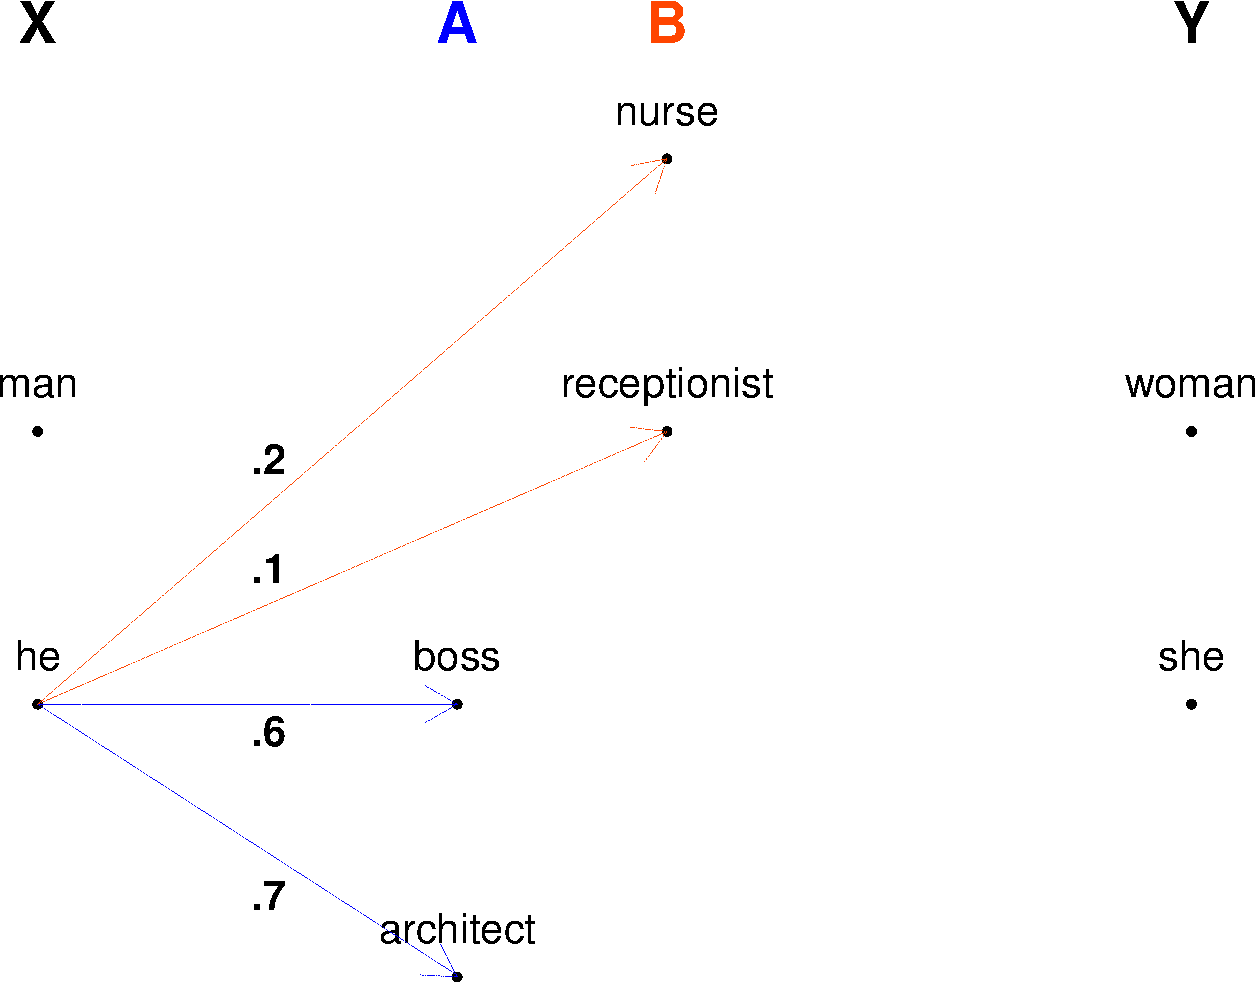
\includegraphics[width=1\linewidth]{_main_files/figure-latex/unnamed-chunk-2-1} \end{center}

\normalsize

The first impression is that while there is a shift for associated words
towards smaller cosine distances as compared to the neutral words,
slightly surprisingly a slightly weaker shift in the same direction is
visible for attributes associated with different stereotypes. Moreover,
the empirical distributions overlap to alarge extent and the means
grouped by connection type do not seem too far from each other. In fact,
as there is a lot of variety in the consine distances (as we will soon
see), abd we need to gauge the uncertaintly involved, and to look more
carefully at individual protected words to get a better idea of how the
cosine distance distribution changes for different attribute groups and
different protected classes. Now, let's add the human attributes to the
picture:

\vspace{1mm} \footnotesize

\begin{center}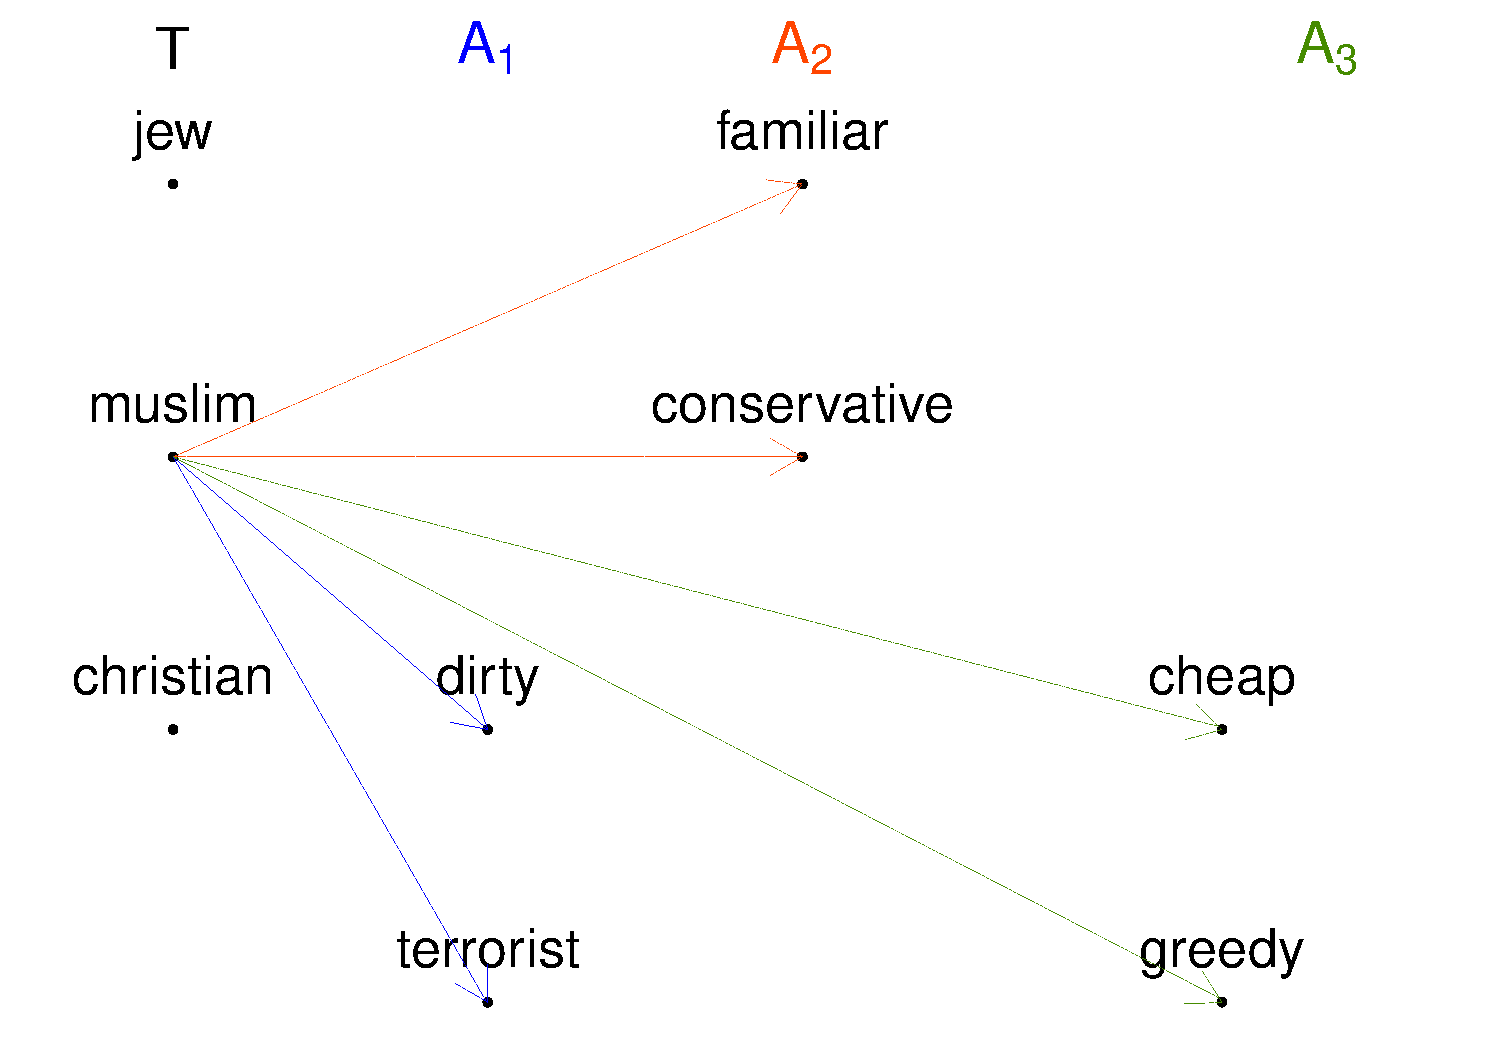
\includegraphics[width=1\linewidth]{_main_files/figure-latex/unnamed-chunk-3-1} \end{center}

\normalsize

\noindent Notice that the distribution for \texttt{human} (even though
we did our best not to include in it any stereotype-related atributes)
is left-skewed, with much overlap with \texttt{associated} and
\texttt{different}, which illustrates the need to take being associated
with humans as an important predictor.

Our focus lies in \texttt{connection} as a predictor. Morever, later on
we'll be interested in looking at the protected words separately, and at
protected words split by connection. For technical reasons it is useful
to represent these factors as integer vectors.

\vspace{1mm} \footnotesize

\begin{Shaded}
\begin{Highlighting}[]
\NormalTok{religion}\OperatorTok{$}\NormalTok{con <-}\StringTok{ }\KeywordTok{as.integer}\NormalTok{(religion}\OperatorTok{$}\NormalTok{connection)}
\NormalTok{religion}\OperatorTok{$}\NormalTok{pw <-}\StringTok{ }\KeywordTok{as.integer}\NormalTok{(religion}\OperatorTok{$}\NormalTok{protectedWord)}
\NormalTok{religion}\OperatorTok{$}\NormalTok{pwFactor <-}\StringTok{ }\KeywordTok{factor}\NormalTok{(}\KeywordTok{paste0}\NormalTok{(religion}\OperatorTok{$}\NormalTok{protectedWord, religion}\OperatorTok{$}\NormalTok{connection))}
\NormalTok{religion}\OperatorTok{$}\NormalTok{pwIndex <-}\StringTok{ }\KeywordTok{as.integer}\NormalTok{(religion}\OperatorTok{$}\NormalTok{pwFactor)}
\end{Highlighting}
\end{Shaded}

\normalsize

A short script, \texttt{cleanDataset} to make this faster, so
equivalently:

\vspace{1mm} \footnotesize

\begin{Shaded}
\begin{Highlighting}[]
\KeywordTok{source}\NormalTok{(}\StringTok{"../functions/cleanDataset.R"}\NormalTok{)}
\NormalTok{religion <-}\StringTok{ }\KeywordTok{read.csv}\NormalTok{(}\StringTok{"../datasets/religionReddit.csv"}\NormalTok{)[}\OperatorTok{-}\DecValTok{1}\NormalTok{]}
\NormalTok{religion <-}\StringTok{ }\KeywordTok{cleanDataset}\NormalTok{(religion,}\KeywordTok{c}\NormalTok{(}\StringTok{"christian"}\NormalTok{,}\StringTok{"human"}\NormalTok{,}\StringTok{"jewish"}\NormalTok{,}\StringTok{"muslim"}\NormalTok{,}\StringTok{"neutral"}\NormalTok{))}
\end{Highlighting}
\end{Shaded}

\normalsize

For now, let's focus on five protected words related to islam (``imam'',
``islam'', ``mosque'', ``muslim'', and ``quran''). The word list
associates with islam four stereotypical attributes (``violent'',
``terrorist'', ``uneducated'' and ``dirty''). First, we select and plot
the empirical distributions for these protected words.

\vspace{1mm} \footnotesize

\begin{Shaded}
\begin{Highlighting}[]
\KeywordTok{library}\NormalTok{(tidyverse)}
\NormalTok{muslimWords <-}\StringTok{ }\KeywordTok{c}\NormalTok{(}\StringTok{"imam"}\NormalTok{,}\StringTok{"islam"}\NormalTok{,}\StringTok{"mosque"}\NormalTok{,}\StringTok{"muslim"}\NormalTok{,}\StringTok{"quran"}\NormalTok{)}
\NormalTok{muslim <-}\StringTok{ }\NormalTok{religion }\OperatorTok\StringTok{ }\KeywordTok{filter}\NormalTok{(protectedWord }\OperatorTok\StringTok{ }\NormalTok{muslimWords)}
\KeywordTok{ggplot}\NormalTok{(muslim, }\KeywordTok{aes}\NormalTok{(}\DataTypeTok{x =}\NormalTok{  cosineDistance, }\DataTypeTok{fill =}\NormalTok{ connection, }\DataTypeTok{color =}\NormalTok{ connection))}\OperatorTok{+}
\StringTok{  }\KeywordTok{geom_density}\NormalTok{(}\DataTypeTok{alpha=}\FloatTok{0.6}\NormalTok{,}\DataTypeTok{size =} \FloatTok{.2}\NormalTok{)}\OperatorTok{+}\StringTok{ }
\StringTok{  }\KeywordTok{scale_fill_manual}\NormalTok{(}\DataTypeTok{values =} \KeywordTok{c}\NormalTok{(}\StringTok{"orangered4"}\NormalTok{,}\StringTok{"chartreuse4"}\NormalTok{, }\StringTok{"skyblue"}\NormalTok{, }\StringTok{"gray"}\NormalTok{))}\OperatorTok{+}
\StringTok{  }\KeywordTok{scale_x_continuous}\NormalTok{(}\DataTypeTok{breaks =} \KeywordTok{seq}\NormalTok{(}\FloatTok{0.3}\NormalTok{,}\FloatTok{1.5}\NormalTok{, }\DataTypeTok{by =} \FloatTok{0.1}\NormalTok{))}\OperatorTok{+}\KeywordTok{xlab}\NormalTok{(}\StringTok{"cosine distance"}\NormalTok{)}\OperatorTok{+}
\StringTok{  }\KeywordTok{scale_color_manual}\NormalTok{(}\DataTypeTok{values =} \KeywordTok{c}\NormalTok{(}\StringTok{"orangered4"}\NormalTok{,}\StringTok{"chartreuse4"}\NormalTok{,}\StringTok{"skyblue"}\NormalTok{,}\StringTok{"gray"}\NormalTok{))}\OperatorTok{+}
\StringTok{  }\KeywordTok{theme_tufte}\NormalTok{()}\OperatorTok{+}\KeywordTok{ggtitle}\NormalTok{(}\StringTok{"Empirical distribution of distances (muslim)"}\NormalTok{)}
\end{Highlighting}
\end{Shaded}

\begin{center}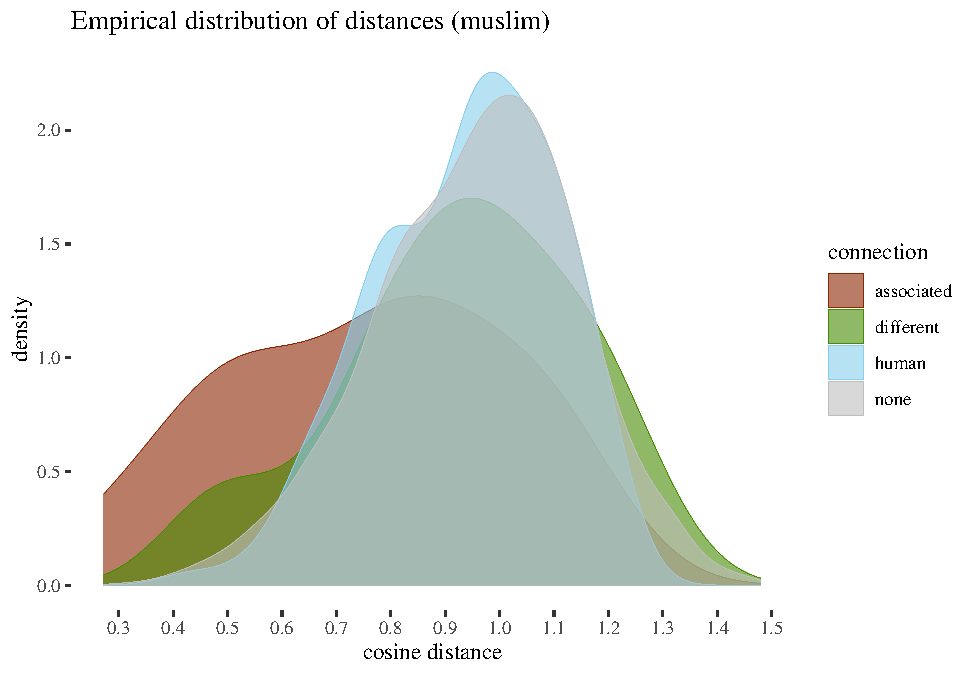
\includegraphics[width=1\linewidth]{_main_files/figure-latex/unnamed-chunk-6-1} \end{center}

\normalsize

\noindent Once we focus on words related to islam, the associated bias
seems to be stronger than in the whole dataset. This is a step towards
illustrating that the distribution of bias is uneven.

Now, say we want to look at a single protected word. Since the dataset
also contains comparison multiple control neutral and human attributes,
we randomly select only 5 from \texttt{none} and 5 from \texttt{human}
control groups of those for the visualisation purposes.

\vspace{1mm} \footnotesize

\begin{Shaded}
\begin{Highlighting}[]
\KeywordTok{library}\NormalTok{(tidyverse)}
\NormalTok{muslimClass <-}\StringTok{ }\NormalTok{muslim }\OperatorTok\StringTok{ }\KeywordTok{filter}\NormalTok{(protectedWord }\OperatorTok{==}\StringTok{ "muslim"}\NormalTok{)}
\NormalTok{neutralSample <-}\StringTok{ }\KeywordTok{sample_n}\NormalTok{(}\KeywordTok{filter}\NormalTok{(muslimClass,connection }\OperatorTok{==}\StringTok{ "none"}\NormalTok{), }\DecValTok{5}\NormalTok{)}
\NormalTok{humanSample <-}\StringTok{ }\KeywordTok{sample_n}\NormalTok{(}\KeywordTok{filter}\NormalTok{(muslimClass,connection }\OperatorTok{==}\StringTok{ "human"}\NormalTok{), }\DecValTok{5}\NormalTok{)}
\NormalTok{muslimVis <-}\StringTok{ }\NormalTok{muslimClass }\OperatorTok\StringTok{ }\KeywordTok{filter}\NormalTok{(connection }\OperatorTok{!=}\StringTok{ "none"} \OperatorTok{&}\StringTok{ }\NormalTok{connection }\OperatorTok{!=}\StringTok{"human"}\NormalTok{)}
\NormalTok{muslimVis <-}\StringTok{ }\KeywordTok{rbind}\NormalTok{(muslimVis,neutralSample,humanSample)}

\CommentTok{#we plug in our visualisation script}
\KeywordTok{source}\NormalTok{(}\StringTok{"../functions/visualisationTools.R"}\NormalTok{)}
\CommentTok{#two arguments: dataset and protected word}
\KeywordTok{visualiseProtected}\NormalTok{(muslimVis,}\StringTok{"muslim"}\NormalTok{)}
\end{Highlighting}
\end{Shaded}

\begin{center}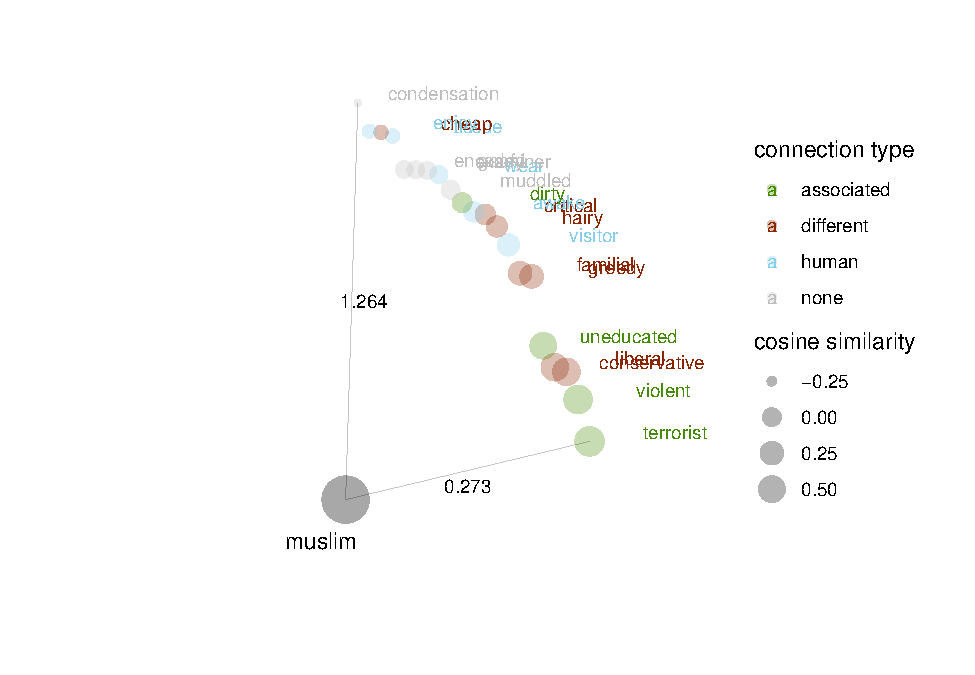
\includegraphics[width=1\linewidth]{_main_files/figure-latex/tableMuslimActive-1} \end{center}

\normalsize

Note that the distance between the grey point and the other points is
proportional to cosine distance, the non-grey point size is proportional
to cosine similarity to the protected word, and color groups by the
connection type. So for \texttt{muslim} it seems that the stereotypes
coming from the word list are fairly well visible. To give you some
taste of how uneven the dataset is, compare this to what happens with
\texttt{priest}.

\vspace{1mm} \footnotesize

\begin{Shaded}
\begin{Highlighting}[]
\KeywordTok{library}\NormalTok{(tidyverse)}
\NormalTok{priestClass <-}\StringTok{ }\NormalTok{religion }\OperatorTok\StringTok{ }\KeywordTok{filter}\NormalTok{(protectedWord }\OperatorTok{==}\StringTok{ "priest"}\NormalTok{)}
\NormalTok{neutralSample <-}\StringTok{ }\KeywordTok{sample_n}\NormalTok{(}\KeywordTok{filter}\NormalTok{(priestClass,connection }\OperatorTok{==}\StringTok{ "none"}\NormalTok{), }\DecValTok{5}\NormalTok{)}
\NormalTok{humanSample <-}\StringTok{ }\KeywordTok{sample_n}\NormalTok{(}\KeywordTok{filter}\NormalTok{(priestClass,connection }\OperatorTok{==}\StringTok{ "human"}\NormalTok{), }\DecValTok{5}\NormalTok{)}
\NormalTok{priestVis <-}\StringTok{ }\NormalTok{priestClass }\OperatorTok\StringTok{ }\KeywordTok{filter}\NormalTok{(connection }\OperatorTok{!=}\StringTok{ "none"} \OperatorTok{&}\StringTok{ }\NormalTok{connection }\OperatorTok{!=}\StringTok{"human"}\NormalTok{)}
\NormalTok{priestVis <-}\StringTok{ }\KeywordTok{rbind}\NormalTok{(priestVis,neutralSample,humanSample)}

\CommentTok{#we plug in our visualisation script}
\KeywordTok{source}\NormalTok{(}\StringTok{"../functions/visualisationTools.R"}\NormalTok{)}
\CommentTok{#two arguments: dataset and protected word}
\KeywordTok{visualiseProtected}\NormalTok{(priestVis,}\StringTok{"priest"}\NormalTok{)}
\end{Highlighting}
\end{Shaded}

\begin{center}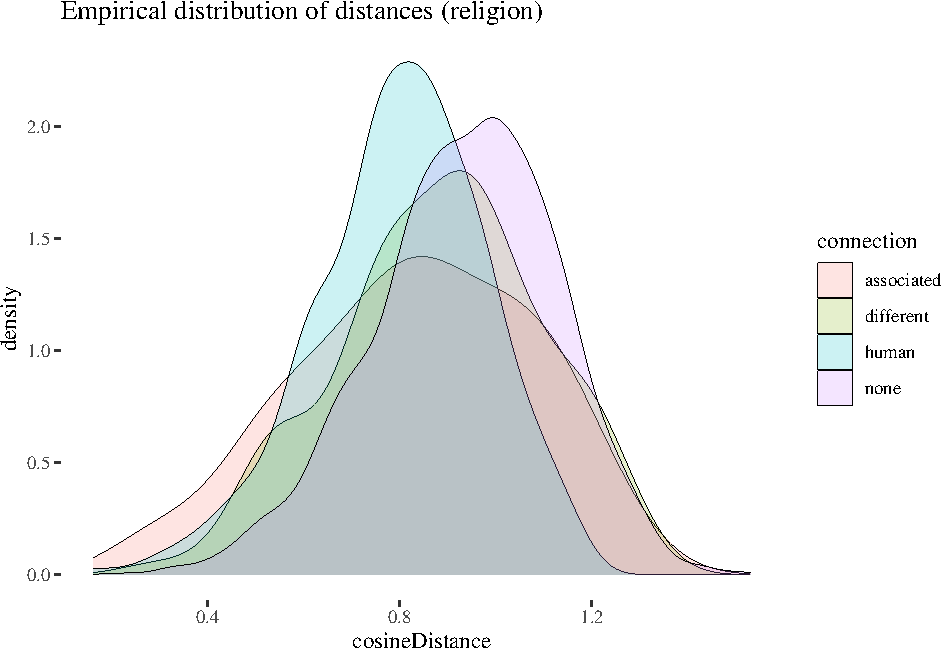
\includegraphics[width=1\linewidth]{_main_files/figure-latex/unnamed-chunk-7-1} \end{center}

\normalsize

\noindent Here you can see that some human attributes are closer than
stereotype attributes, and that there is no clear reason to claim that
\texttt{associated} attributes are closer than \texttt{different} or
\texttt{human} attributes. This, again, illustrates the need of
case-by-case analysis with control groups.

The general idea now is that the word lists provided in different pieces
of research are just samples of attributes associates with various
stereotypes and should be treated as such: the uncertaintly involved and
the sample sizes should have clear impact on our estimates.

We will now think of cosine distance as the output variable, and will
build a few bayesian models to compare. First, we just build a baseline
model which estimates cosine distance to the attributes separately for
each protected word. The underlying idea is that different protected
words migh in general have different relations to all the attributes and
this relations should be our point of departure.

Here is the intution behind the mathematical Bayesian model involved.
Our outcome variable is \texttt{cosine\ difference}, which we take to me
normally distributed around the predicted mean for a given protected
word (that is, we assume the residuals are normally distributed). The
simplest model specification is:

\begin{align}
cosineDistance_i  & \sim dnorm(\mu_i, \sigma) \\
\mu_i & = m_{pw} \\
m_{pw} & ~ dnorm(1,.5) \\
\sigma &\sim  dcauchy(0,1)
\end{align}

That is, we assume the estimated means might be different for diferent
protected words and our prior for the mean and the overal standard
deviation are normal with mean 1 and sd=.5 and half-cauchy with
parameters \texttt{0,1}. Further on we'll also estimate additional
impact the connection type may have. For this impact we take a slightly
skeptical prior centered around 0 distributed normally with sd = 1.
These are fairly weak and slightly skeptical regularizing priors, which
can be illustrated as follows:

\vspace{2mm}

\begin{center}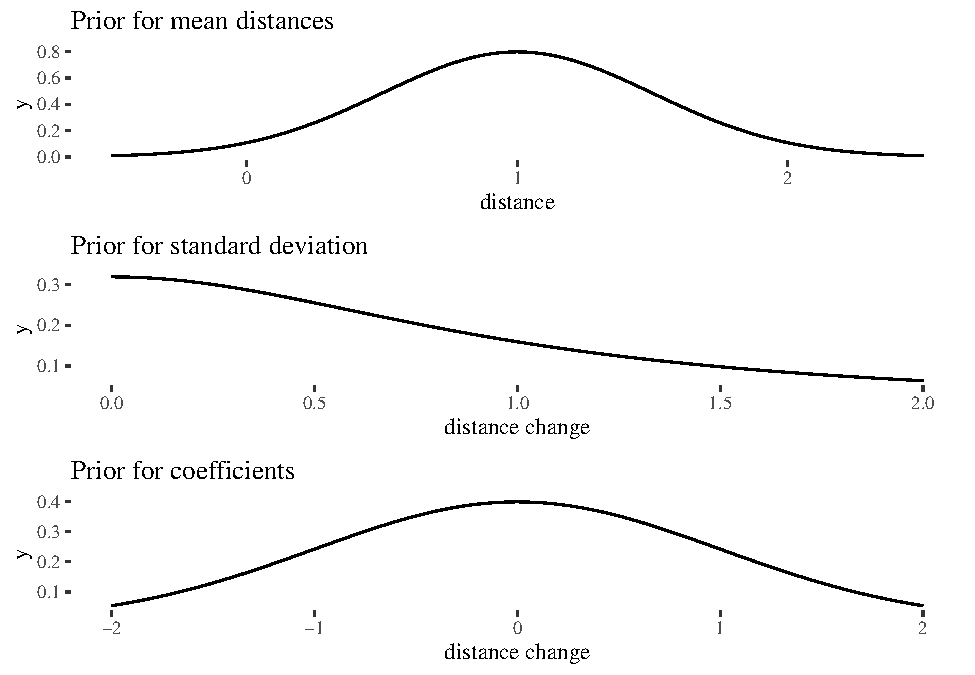
\includegraphics[width=1\linewidth]{_main_files/figure-latex/priorsVis-1} \end{center}

Now we can define and compile the baseline model. Its parameters will
have a posterior distribution obtained using either Hamiltionian Monte
Carlo methods (STAN) available through the \texttt{rethinking} package.

\vspace{1mm} \footnotesize

\begin{Shaded}
\begin{Highlighting}[]
\KeywordTok{library}\NormalTok{(rethinking)}
\KeywordTok{options}\NormalTok{(}\DataTypeTok{buildtools.check =} \ControlFlowTok{function}\NormalTok{(action) }\OtherTok{TRUE}\NormalTok{ )}
\NormalTok{religionBaseline <-}\StringTok{ }\KeywordTok{ulam}\NormalTok{(}
  \KeywordTok{alist}\NormalTok{(}
\NormalTok{    cosineDistance }\OperatorTok{~}\StringTok{ }\KeywordTok{dnorm}\NormalTok{(mu,sigma),}
\NormalTok{    mu <-}\StringTok{ }\NormalTok{m[pw],}
\NormalTok{    m[pw] }\OperatorTok{~}\StringTok{ }\KeywordTok{dnorm}\NormalTok{(}\DecValTok{1}\NormalTok{,.}\DecValTok{5}\NormalTok{),}
\NormalTok{    sigma }\OperatorTok{~}\StringTok{ }\KeywordTok{dcauchy}\NormalTok{(}\DecValTok{0}\NormalTok{,}\DecValTok{1}\NormalTok{)}
\NormalTok{  ),}
  \DataTypeTok{data =}\NormalTok{ religion,}
  \DataTypeTok{chains=}\DecValTok{2}\NormalTok{ , }\DataTypeTok{iter=}\DecValTok{4000}\NormalTok{ , }\DataTypeTok{warmup=}\DecValTok{1000}\NormalTok{,}
  \DataTypeTok{start=} \KeywordTok{list}\NormalTok{(}\DataTypeTok{mu =} \DecValTok{1}\NormalTok{, }\DataTypeTok{co =} \DecValTok{0}\NormalTok{, }\DataTypeTok{sigma=} \FloatTok{.3}\NormalTok{),}
  \DataTypeTok{log_lik =} \OtherTok{TRUE}\NormalTok{, }\DataTypeTok{cores=}\DecValTok{4}
\NormalTok{)}
\CommentTok{#saving}
\CommentTok{#saveRDS(religionBaseline, }
\CommentTok{#file = "cosineAnalysis/models/religionBaseline.rds")}
\end{Highlighting}
\end{Shaded}

The only reason we need it is the evaluation of connection as a
predictor. Does including it in o the model improve the situation? To
investigate this, let's now build a model according to the following
specification:

\begin{align}
cosineDistance_i  & \sim dnorm(\mu_i, \sigma) \\
\mu_i & = m_{pw} + co_{con}\\
m_{pw} & ~ dnorm(1,.5) \\
co_{con} & ~ dnorm(0,1) \\
\sigma &\sim  dcauchy(0,1)
\end{align}

\noindent The idea now is that each connection type comes with its own
coefficient \(co\) that has impact on mean distances for protected words
taken separately.

\vspace{1mm} \footnotesize

\begin{Shaded}
\begin{Highlighting}[]
\KeywordTok{library}\NormalTok{(rethinking)}
\KeywordTok{options}\NormalTok{(}\DataTypeTok{buildtools.check =} \ControlFlowTok{function}\NormalTok{(action) }\OtherTok{TRUE}\NormalTok{ )}
\NormalTok{religionCoefs <-}\StringTok{ }\KeywordTok{ulam}\NormalTok{(}
  \KeywordTok{alist}\NormalTok{(}
\NormalTok{    cosineDistance }\OperatorTok{~}\StringTok{ }\KeywordTok{dnorm}\NormalTok{(mu,sigma),}
\NormalTok{    mu <-}\StringTok{ }\NormalTok{m[pw] }\OperatorTok{+}\StringTok{ }\NormalTok{co[con],}
\NormalTok{    m[pw] }\OperatorTok{~}\StringTok{ }\KeywordTok{dnorm}\NormalTok{(}\DecValTok{1}\NormalTok{,.}\DecValTok{5}\NormalTok{),}
\NormalTok{    co[con] }\OperatorTok{~}\KeywordTok{dnorm}\NormalTok{(}\DecValTok{0}\NormalTok{,.}\DecValTok{5}\NormalTok{),}
\NormalTok{    sigma }\OperatorTok{~}\StringTok{ }\KeywordTok{dcauchy}\NormalTok{(}\DecValTok{0}\NormalTok{,}\DecValTok{1}\NormalTok{)}
\NormalTok{  ),}
  \DataTypeTok{data =}\NormalTok{ religion,}
  \DataTypeTok{chains=}\DecValTok{2}\NormalTok{ , }\DataTypeTok{iter=}\DecValTok{8000}\NormalTok{ , }\DataTypeTok{warmup=}\DecValTok{1000}\NormalTok{, }
  \DataTypeTok{log_lik =} \OtherTok{TRUE}
\NormalTok{)}
\end{Highlighting}
\end{Shaded}

\normalsize

\noindent First, let's see if this model is really better in terms of
the Widely Acceptable Information Criterion (WAIC):

\vspace{1mm} \footnotesize

\begin{Shaded}
\begin{Highlighting}[]
\CommentTok{#the calculation requires models which are large, we prepared the table}
\CommentTok{#compareBaseline <- print(round(compare(religionBaseline, religionCoefs)), 3)}
\NormalTok{compareBaseline <-}\StringTok{ }\KeywordTok{readRDS}\NormalTok{(}\StringTok{"../datasets/compareBaseline.rds"}\NormalTok{)}
\NormalTok{compareBaseline}
\end{Highlighting}
\end{Shaded}

\begin{verbatim}
##                   WAIC SE dWAIC dSE pWAIC weight
## religionCoefs    -2328 93     0  NA    20      1
## religionBaseline -2283 95    45  17    16      0
\end{verbatim}

\normalsize

\end{document}
